\section{Introdução}

\subsection{Contextualização}

\begin{frame}{Motivação}
    \begin{columns}
        \begin{column}{0.5\textwidth}
            \begin{itemize}%[<+->]
                \item Remédios de uso contínuo;
                \item Maior longevidade da população;
                \item Problemas de visão em idade avançada (presbiopia);
                \item Embalagens semelhantes confundem pacientes;
                \item O uso indevido de medicamentos tende a ser prejudicial à saúde.
            \end{itemize}
        \end{column}
        \begin{column}{0.5\textwidth}
            \begin{figure}
                \centering
                \caption*{Diagrama de Snellen, fora de escala.}
                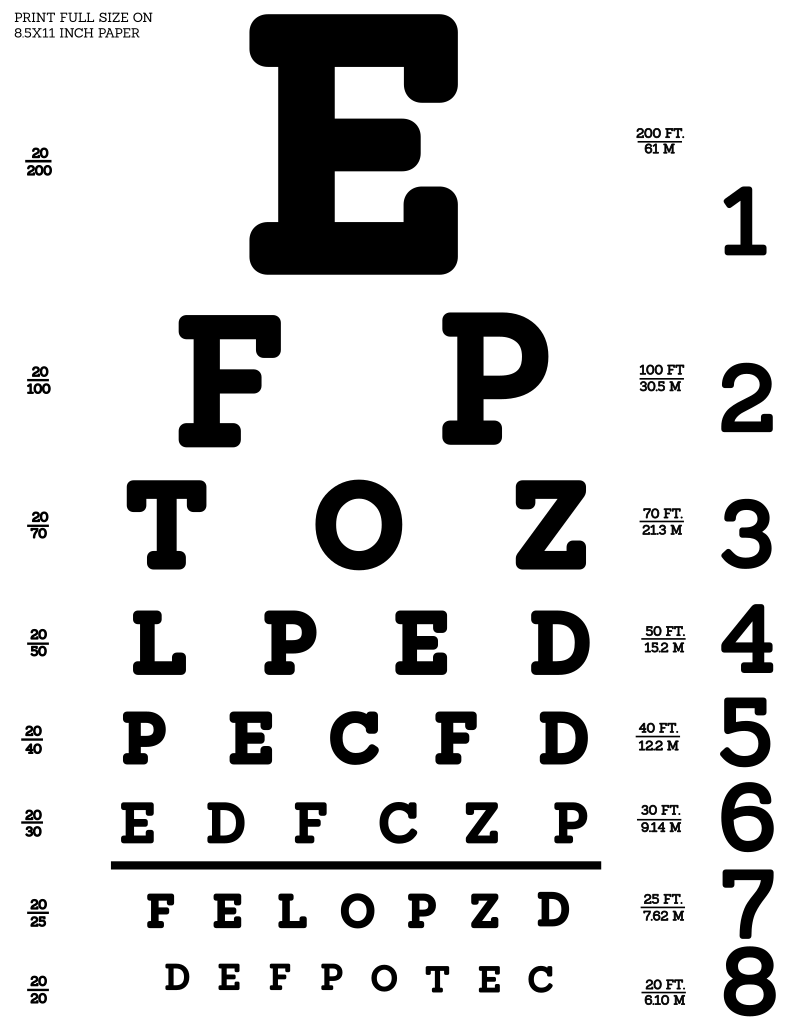
\includegraphics[keepaspectratio, width=\linewidth, height=0.65\textheight]{../pictures/Snellen_chart.png}
                \caption*{Fonte: \href{https://commons.wikimedia.org/wiki/File:Snellen_chart_by_Openclipart.svg}{Openclipart, CC0, via Wikimedia Commons}}
            \end{figure}
        \end{column}
    \end{columns}
\end{frame}

\subsection{Objetivos}
\begin{frame}{Objetivos}
    \begin{itemize}%[<+->]
        \item Sistema capaz de identifcar embalagens de medicamentos;
        \item Carregar arquivos de bulas eletrônicas;
        \item Baseado em visão computacional;
        \item Lidar com diferentes imagens.
    \end{itemize}
\end{frame}
